
\subsection{Speedup across four benchmarks}
\label{app:detail:results4}

\begin{table}[t]
\centering
\caption{\textbf{Whole-task end-to-end speedup of LEAP: four benchmarks, three draft sizes, two targets} (one H100
shared by target and draft; $\tau^2$-bench and BFCL execute tools; 63, 60, 40 and 60 test tasks). Each benchmark
serves its three drafts in one configuration (App.~\ref{app:serving}). Agreement is the draft's offline exact-match rate (\%) on the
target's held-out contexts (BFCL: decision level); acceptance is the share of verified proposals that were
accepted in the runs (the per-proposal rate of Table~\ref{tab:agree}); $c$ is the measured number of committed steps per round (Eq.~\ref{eq:c}); the 95\% interval is a
task-level bootstrap of the pooled ratio (10{,}000 resamples). Bold marks the fastest of the three drafts for
a benchmark and target. Task success per arm shows no systematic change (App.~\ref{app:success}).}
\label{tab:four}
\footnotesize\setlength{\tabcolsep}{4pt}\renewcommand{\arraystretch}{0.92}
\begin{tabular}{llrrrrrrrc}
\toprule
benchmark & draft & steps & $t_{\mathrm{gen}}$ (s) & $k$ & agreem. & accept. & $c$ & speedup & 95\% CI \\
\midrule
\multicolumn{10}{l}{\emph{Target Qwen3-32B}} \\
\midrule
\multirow{3}{*}{OpenAGI} & 0.6B & 4.2  & 1.1  & 3 & 75.4 & 0.75 & 2.05 & 1.50\xx{} & [1.36, 1.65] \\
                & 1.7B & 4.2  & 1.1  & 3 & 77.6 & 0.78 & 2.18 & \textbf{1.55\xx{}} & [1.43, 1.68] \\
                & 4B   & 4.2  & 1.1  & 3 & 78.7 & 0.79 & 2.26 & 1.46\xx{} & [1.30, 1.62] \\
\cmidrule(lr){2-10}
\multirow{3}{*}{TaskBench} & 0.6B & 5.0  & 1.8  & 3 & 74.7 & 0.70 & 1.94 & 1.38\xx{} & [1.24, 1.55] \\
                & 1.7B & 5.0  & 1.8  & 3 & 81.0 & 0.76 & 2.07 & \textbf{1.47\xx{}} & [1.34, 1.61] \\
                & 4B   & 5.0  & 1.8  & 3 & 80.5 & 0.75 & 2.11 & 1.36\xx{} & [1.22, 1.52] \\
\cmidrule(lr){2-10}
\multirow{3}{*}{$\tau^2$-bench} & 0.6B & 13.9 & 12.4 & 2 & 63.3 & 0.65 & 1.92 & 1.61\xx{} & [1.44, 1.79] \\
                & 1.7B & 13.9 & 12.5 & 2 & 68.1 & 0.63 & 1.88 & \textbf{1.63\xx{}} & [1.46, 1.81] \\
                & 4B   & 13.9 & 12.4 & 2 & 69.5 & 0.66 & 1.90 & 1.56\xx{} & [1.43, 1.73] \\
\cmidrule(lr){2-10}
\multirow{3}{*}{BFCL multi-turn} & 0.6B & 10.1 & 10.8 & 2 & 66.7 & 0.53 & 1.44 & 1.18\xx{} & [1.08, 1.28] \\
                & 1.7B & 10.1 & 10.8 & 2 & 72.7 & 0.59 & 1.55 & 1.28\xx{} & [1.20, 1.36] \\
                & 4B   & 10.1 & 10.8 & 2 & 79.8 & 0.65 & 1.67 & \textbf{1.34\xx{}} & [1.21, 1.48] \\
\midrule
\multicolumn{10}{l}{\emph{Target Gemma-4-31B-it}} \\
\midrule
\multirow{3}{*}{OpenAGI} & 0.6B & 4.3  & 2.1 & 3 & 79.8 & 0.78 & 2.18 & \textbf{1.55\xx{}} & [1.35, 1.79] \\
                & 1.7B & 4.3  & 2.1 & 3 & 77.3 & 0.75 & 2.08 & \textbf{1.55\xx{}} & [1.35, 1.78] \\
                & 4B   & 4.3  & 2.1 & 3 & 79.9 & 0.76 & 2.15 & 1.52\xx{} & [1.34, 1.73] \\
\cmidrule(lr){2-10}
\multirow{3}{*}{TaskBench} & 0.6B & 4.9  & 2.3 & 3 & 80.1 & 0.82 & 2.30 & 1.60\xx{} & [1.47, 1.76] \\
                & 1.7B & 4.9  & 2.3 & 3 & 84.6 & 0.83 & 2.43 & \textbf{1.68\xx{}} & [1.56, 1.82] \\
                & 4B   & 4.9  & 2.3 & 3 & 84.2 & 0.85 & 2.45 & 1.62\xx{} & [1.51, 1.75] \\
\cmidrule(lr){2-10}
\multirow{3}{*}{$\tau^2$-bench} & 0.6B & 14.7 & 4.7 & 2 & 72.8 & 0.80 & 2.27 & \textbf{1.63\xx{}} & [1.50, 1.77] \\
                & 1.7B & 14.7 & 4.7 & 2 & 76.4 & 0.79 & 2.20 & 1.55\xx{} & [1.44, 1.67] \\
                & 4B   & 14.7 & 4.7 & 2 & 77.6 & 0.80 & 2.24 & 1.55\xx{} & [1.43, 1.67] \\
\cmidrule(lr){2-10}
\multirow{3}{*}{BFCL multi-turn} & 0.6B & 10.2 & 3.3 & 2 & 63.6 & 0.50 & 1.41 & 1.10\xx{} & [1.04, 1.16] \\
                & 1.7B & 10.2 & 3.3 & 2 & 69.7 & 0.55 & 1.48 & 1.12\xx{} & [1.06, 1.18] \\
                & 4B   & 10.2 & 3.3 & 2 & 74.7 & 0.66 & 1.66 & \textbf{1.16\xx{}} & [1.09, 1.23] \\
\bottomrule
\end{tabular}
\end{table}

Table~\ref{tab:four} summarizes the four benchmarks for drafts of 0.6B, 1.7B and 4B parameters
trained with one recipe, with Qwen3-32B and with Gemma-4-31B-it as the target. The Gemma rows repeat the
whole pipeline: new sequential traces on the same task splits, the same three drafts trained with the same
recipe on those traces, and the same serving configurations (App.~\ref{app:serving} gives the two serving
details that differ).

With the smallest draft, trained for GPU-minutes on the target's own traces, LEAP speeds up whole tasks by
1.18--1.61\xx{} with Qwen3 and 1.10--1.63\xx{} with Gemma, on planning-only tasks and on tasks that execute
tools. Task success shows no systematic change: across the 28 comparisons of App.~\ref{app:success}, the
speculative arm solves more tasks in 8, fewer in 8 and as many in 12, never differing by more than three.
Every committed action is target-authored, but whole trajectories can differ from the target-only run: they
are identical on 96\% of the OpenAGI and 83\% of the TaskBench tasks, while on the tool benchmarks, whose
steps reason for 10--12\,s, most trajectories take a different decision at some step (Table~\ref{tab:parity}).
On $\tau^2$-bench 37 of the 40 tasks are still scored identically by both arms with Qwen3, and with Gemma the
two arms follow identical trajectories on 52--55 of the 60--63 planning tasks. Repeating the $\tau^2$-bench main run (the
configuration of Table~\ref{tab:model}) end to end gives 1.59\xx{} [1.44, 1.77] against 1.58\xx{}
[1.44, 1.75] in the first pass.

The model of Sec.~\ref{sec:model} explains the ordering across benchmarks and the differences between the
targets. OpenAGI has the highest acceptance and $k{=}3$, so it commits the most steps per round
($c{=}2.05$ with Qwen3), but it also pays the largest end-of-task loss ($e{=}0.38$; tasks are 4 steps
long). $\tau^2$-bench has lower acceptance but long tasks ($e{=}0.11$) and a draft that is cheap next to a
12\,s target step ($k\,t_{\mathrm{draft}}/t_{\mathrm{gen}} = 0.03$). BFCL is limited by structure: its
segments between user turns average 2.6 steps, 26\% of its rounds are width-1 hand-off probes at turn
boundaries, and its second proposal is accepted in only 7\% of rounds, so $c$ is 1.44 and the ceiling
$\min(k{+}1, L)/\beta$ is about 1.7\xx{} even for a perfect draft. Changing the target changes the step
length, and with it the weight of the draft's cost. Gemma's steps are about twice as long as Qwen3's on the
planning benchmarks (2.1 and 2.3\,s against 1.1 and 1.8\,s), which lowers the draft term at a fixed draft
cost, and its drafts agree with it more often (77--85\% against 75--81\%), so its planning speedups are
higher (1.52--1.68\xx{}). Its tool steps are shorter: 2.6 times on $\tau^2$-bench (4.7 against 12.4\,s) and
three times on BFCL (3.3 against 10.8\,s). There the draft term rises from 0.03--0.04 to 0.08--0.12 and
from 0.04--0.07 to 0.11--0.19: on $\tau^2$-bench, with acceptance flat across sizes (0.79--0.80), the
smallest draft is the fastest, and on BFCL the speedups fall to 1.10--1.16\xx{} while the turn structure
that bounds the ceiling is unchanged.

The draft size follows the same logic. With Qwen3 the 1.7B draft is faster on every benchmark
(1.28--1.63\xx{}) and the 4B draft is faster still on BFCL alone. With Gemma the three drafts tie on
OpenAGI (1.55, 1.55 and 1.52\xx{}), where the ratio of committed steps between sizes is 1.00 against a cost
ratio of 1.01; the 1.7B draft is fastest on TaskBench and the 4B draft on BFCL, as with Qwen3.
Sec.~\ref{sec:training} takes this up.

In the $\tau^2$-bench main run of Table~\ref{tab:model}, two tasks end early in the speculative arm (the
re-measurement of Table~\ref{tab:four} has no such case: 40 of 40 terminate). On one context that six
test tasks share, the target, verifying three prefixes in one batch, ran to its
2{,}048-token budget without emitting an action in two of them, while the same
context parsed in the sequential arm and in the other four tasks. We attribute this to the
target's batch-dependent decoding (App.~\ref{app:success}); the commit audit passes on both tasks. The two tasks
are kept in the pooled ratio (their speculative arm is shorter), and excluding
them gives 1.58\xx{} [1.44, 1.75] as well.

\subsection{Framework validation}
\label{app:detail:validation}\label{app:validation}

We test Eq.~\ref{eq:S} as a predictor. For each configuration we take
$c$ from the measured per-position hit rates (Eq.~\ref{eq:c}), replay the
\emph{sequential} arm's per-step generation times to obtain $\beta$ (group
consecutive steps of a segment into rounds with independent hits at rate $q_1$
and take the maximum within each group), and measure $t_{\mathrm{draft}}$. The
prediction uses no timing from the speculative arm's verifications; the hit rates and the draft time are
measured in the speculative run.
Table~\ref{tab:model}, Table~\ref{tab:tool} and Fig.~\ref{fig:pred}(a) compare it with the measured
pooled speedup for twenty-one configurations spanning acceptance $0.02$--$0.79$, depth
$k \in \{1,2,3,5\}$, normalized proposing cost $D \in [0.02, 0.74]$ and added
tool latency up to $0.46$ of a target step.


\begin{figure}[tbp]
\centering
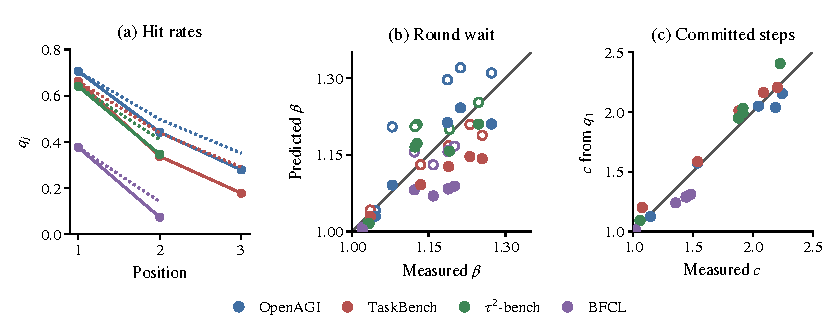
\includegraphics[width=\linewidth]{figures/fig_prediction_components.pdf}
\caption{\textbf{Component checks of the latency framework.} (a) Measured per-position hit rates (solid)
and $q_1^j$ (dotted) for the four main configurations. (b) Trace-replay $\beta$ (filled) and the
independent-step closed form (hollow), against measured values. (c) Committed steps from the
single-rate replay against measured commits. Configuration details are in Table~\ref{tab:model}.}
\label{fig:components}
\end{figure}


\begin{table}[t]
\centering
\footnotesize
\caption{\textbf{Predicted vs.\ measured speedup.} $q_j$: measured
per-position hit rates; $c$: committed steps per round; $\beta$: round-wait
inflation, predicted from the sequential arm's step times and measured from
the speculative arm; draft: the measured draft time per round divided by the
mean sequential step time (the $D$ term of Eq.~\ref{eq:S}, with rounds that
stop proposing early counted as run). ``i.i.d.''
replaces the measured hit rates by $q_j = q_1^{\,j}$. Every row was run with
cancellation, so the harness never waits on already-discarded verifications
(Sec.~\ref{sec:model}, assumption (e)) and the measured column is the speedup as run.
Rows with other $k$ exercise the depth terms of the model; Table~\ref{tab:tool} exercises its tool
terms. The 32B-direct rows use the target
itself, with reasoning disabled, as the draft; the untrained rows use the 0.6B base without an adapter.
A dash marks a position beyond the row's $k$.}
\label{tab:model}
\setlength{\tabcolsep}{3.2pt}
\resizebox{\linewidth}{!}{%
\begin{tabular}{llrrrrrrrrrrr}
\toprule
 & & & \multicolumn{3}{c}{hit rates} & & \multicolumn{2}{c}{$\beta$} & & \multicolumn{2}{c}{predicted} & \\
\cmidrule(lr){4-6}\cmidrule(lr){8-9}\cmidrule(lr){11-12}
benchmark & draft & $k$ & $q_1$ & $q_2$ & $q_3$ & $c$ & pred. & meas. & draft & i.i.d. & Eq.~\ref{eq:S} & measured \\
\midrule
OpenAGI   & trained 0.6B   & 1 & 0.74 & --   & --   & 1.54 & 1.09 & 1.08 & 0.08 & 1.35 & 1.32 & 1.34 \\
OpenAGI   & trained 0.6B   & 3 & 0.71 & 0.44 & 0.28 & 2.05 & 1.21 & 1.19 & 0.18 & 1.48 & 1.47 & 1.51 \\
OpenAGI   & trained 0.6B   & 5 & 0.70 & 0.47 & 0.31 & 2.25 & 1.24 & 1.21 & 0.22 & 1.47 & 1.54 & 1.57 \\
OpenAGI   & untrained 0.6B & 3 & 0.15 & 0.00 & 0.00 & 1.14 & 1.03 & 1.05 & 0.13 & 0.97 & 0.98 & 0.98 \\
OpenAGI   & 32B-direct     & 3 & 0.70 & 0.50 & 0.33 & 2.19 & 1.21 & 1.27 & 0.61 & 1.12 & 1.20 & 1.16 \\
\midrule
TaskBench & trained 0.6B   & 1 & 0.72 & --   & --   & 1.54 & 1.09 & 1.13 & 0.08 & 1.36 & 1.32 & 1.27 \\
TaskBench & trained 0.6B   & 3 & 0.66 & 0.34 & 0.18 & 1.88 & 1.13 & 1.19 & 0.16 & 1.56 & 1.46 & 1.37 \\
TaskBench & trained 0.6B   & 5 & 0.67 & 0.37 & 0.22 & 2.09 & 1.14 & 1.25 & 0.21 & 1.60 & 1.55 & 1.41 \\
TaskBench & untrained 0.6B & 3 & 0.21 & 0.04 & 0.00 & 1.07 & 1.03 & 1.04 & 0.07 & 1.10 & 0.98 & 0.98 \\
TaskBench & 32B-direct     & 3 & 0.74 & 0.50 & 0.33 & 2.21 & 1.15 & 1.23 & 0.73 & 1.17 & 1.17 & 1.13 \\
\midrule
$\tau^2$-bench & trained 0.6B & 2 & 0.64 & 0.35 & -- & 1.88 & 1.16 & 1.19 & 0.03 & 1.64 & 1.58 & 1.58 \\
$\tau^2$-bench & trained 0.6B & 3 & 0.71 & 0.37 & 0.27 & 2.23 & 1.21 & 1.25 & 0.04 & 1.92 & 1.78 & 1.79 \\
$\tau^2$-bench & untrained 0.6B & 2 & 0.09 & 0.00 & -- & 1.06 & 1.02 & 1.03 & 0.02 & 1.06 & 1.02 & 1.03 \\
\midrule
BFCL      & trained 0.6B   & 1 & 0.36 & --   & --   & 1.36 & 1.07 & 1.16 & 0.02 & 1.13 & 1.24 & 1.15 \\
BFCL      & trained 0.6B   & 2 & 0.38 & 0.07 & --   & 1.45 & 1.08 & 1.19 & 0.04 & 1.16 & 1.30 & 1.20 \\
BFCL      & trained 0.6B   & 3 & 0.39 & 0.07 & 0.02 & 1.48 & 1.09 & 1.20 & 0.04 & 1.16 & 1.31 & 1.19 \\
BFCL      & untrained 0.6B & 2 & 0.02 & 0.00 & --   & 1.02 & 1.00 & 1.02 & 0.05 & 0.96 & 0.97 & 0.95 \\
\bottomrule
\end{tabular}}
\end{table}

Three observations. First, the prediction is within $0.05$ of the measured
speedup for fourteen of the twenty-one configurations and within $0.10$ for all but
TaskBench at $k{=}5$ ($0.14$; harness idle time removed) and BFCL at $k{=}3$ ($0.12$).
This includes the untrained drafts on all four benchmarks (predicted $0.97$--$1.02$, measured
$0.95$--$1.03$). Second, $\beta$ replayed from sequential step times lands within
$0.07$ of the value measured in the speculative arm on fifteen configurations.
It is $0.08$ below it for the 32B-direct draft on TaskBench, $0.09$--$0.11$ below it on BFCL at
every depth without added latency and at $+2$\,s, whose step times are heavy-tailed (coefficient of
variation 1.07 against 0.3--0.5 elsewhere), and $0.11$ below it on TaskBench at $k{=}5$, where
a round issues up to six verification requests but the target server runs at most four at once
(Table~\ref{tab:serving}), so the last ones wait, which the replay does not model;
the closed form of Sec.~\ref{sec:model} is within $0.13$ on all twenty-one
(Fig.~\ref{fig:components}(b)). The largest speedup errors, TaskBench at $k{=}5$ and
BFCL, are where $\beta$ is under-predicted, which supports assumption (b) only
up to the few percent of concurrency cost the replay does not model. Third, the
i.i.d.\ shortcut $q_j = q_1^{\,j}$ is off by up to $0.18$ in $c$ in either
direction (Fig.~\ref{fig:components}(c)): it over-predicts on TaskBench and $\tau^2$-bench,
where rounds often run into the end of the task so that later positions do not
exist, and under-predicts on BFCL,
where a quarter of the rounds are hand-off probes with no proposal; the paper
therefore reports $q_j$ rather than a single acceptance rate.

\paragraph{Tool latency.}

Adding 2 or 5\,s to every executed tool step, in both arms, exercises the tool terms of Eq.~\ref{eq:S}
(Table~\ref{tab:tool}; 0.16--0.46 of a target step). The speedup falls as tools slow down: from 1.58\xx{} to
1.41\xx{} and 1.20\xx{} on $\tau^2$-bench (40 tasks), and from 1.20\xx{} to 1.07\xx{} and 1.02\xx{} on BFCL
(60 tasks). The hit rates and $c$ barely change, so the loss is in the round cost. The proposals' tools run
while proposing, which raises the draft term from 0.03 to 0.31 and 0.74 on $\tau^2$-bench and from 0.04 to
0.23 and 0.50 on BFCL, and the round pays the delay again when the target executes its own action, while the
sequential arm pays it once per step. For the four points with added latency, Eq.~\ref{eq:S} is within 0.08
of the measured speedup, and within 0.02 with the measured $\beta$; on BFCL it counts only the steps that
execute a tool and only the target's own tool steps (App.~\ref{app:predictor}). Task success, sequential against
speculative, is 22 against 22 and 22 against 27 on $\tau^2$-bench, and 34 against 34 and 34 against 33 on BFCL.

\paragraph{Prediction from offline hit rates.}
Table~\ref{tab:model} takes the hit rates from the run it decomposes. To predict a configuration before
running it, we replay the loop along the held-out sequential trajectories with the draft's teacher-forced
predictions of Table~\ref{tab:offline}: a round proposes up to $k$ actions and stops at a predicted
terminal action, the accepted prefix is the run of consecutive matches, and the round commits $A{+}1$
steps ($A$ when the prefix ends the task). Table~\ref{tab:exante} compares the replayed $q_j$ and $c$
with the live values and feeds them, with the trace-replay $\beta$ and the draft's single-stream
latency measured offline on the same held-out contexts (draft served alone, one request at a time;
0.07 of a target step on the planning benchmarks and 0.014 on $\tau^2$-bench), into Eq.~\ref{eq:S}. On OpenAGI
and $\tau^2$-bench the replay reproduces the live hit rates within 0.05 and predicts the speedup within 0.03;
on $\tau^2$-bench the hit rates come from the 14 validation tasks, sequential timing comes from the 40 test tasks, and draft latency is probed offline. On
TaskBench the replay overestimates $q_1$ (0.73 against 0.66) and the speedup (1.56 against 1.37): the
target's live trajectories depart from its sequential trace on
more tasks there (trajectory parity 0.86 against 0.98 on OpenAGI), and the draft is less accurate on the
contexts the target visits only in the live runs. An ex-ante prediction is therefore accurate to the extent that
the target is trajectory-stable under batched decoding; Proposition~\ref{prop:commit} fixes the
teacher-forced distribution only for the trajectory the target actually takes. Run on the Gemma traces
with offline draft-latency probes for 0.6B and measured per-proposal draft latency from the speculative runs for 1.7B and 4B (Table~\ref{tab:prediction_inputs}), the prediction forecasts 1.64--1.77\xx{} against 1.52--1.68\xx{} measured
on the six planning configurations, high by 0.02--0.21, and 1.60--1.62\xx{} against 1.55--1.63\xx{} on
$\tau^2$-bench, where the replay's lower hit rate on the validation tasks (0.64--0.72 against 0.76--0.77
live) offsets the same $\beta$ gap. That gap is the residual on the planning benchmarks: the trace replay
gives 1.16--1.23 where the measured round-wait inflation is 1.23--1.31. It underestimates
verification wait by 0.05--0.13 across these configurations. This gap does not identify a uniform
per-request slowdown, because the awaited contexts and generation lengths can also change.
For Qwen3 the difference is $-0.03$ to $+0.11$ across Table~\ref{tab:model}; the underlying cause
of the Gemma gap is not established.

\begin{table}[t]
\centering
\caption{\textbf{Ex-ante inputs from teacher-forced predictions.} Hit rates and committed steps per
round from replaying the loop on the held-out sequential trajectories with the offline predictions of
Table~\ref{tab:offline} (``replay''), against the live values of the runs of Table~\ref{tab:model}; the
ex-ante speedup uses the replayed values with the trace-replay $\beta$ and the draft's single-stream
latency measured offline on the held-out contexts. $\tau^2$-bench obtains hit rates from the 14 validation tasks and sequential timing from the 40 test tasks. BFCL is omitted: its
rounds are bounded by user turns with a terminal probe, which the replay does not reproduce. A dash marks
a position beyond $k{=}2$.}
\label{tab:exante}
\small
\begin{tabular}{lrrrrrrrrrr}
\toprule
 & \multicolumn{4}{c}{replay, before the run} & \multicolumn{4}{c}{live, in the run} & \multicolumn{2}{c}{speedup} \\
\cmidrule(lr){2-5}\cmidrule(lr){6-9}\cmidrule(lr){10-11}
benchmark & $q_1$ & $q_2$ & $q_3$ & $c$ & $q_1$ & $q_2$ & $q_3$ & $c$ & ex-ante & measured \\
\midrule
OpenAGI        & 0.70 & 0.45 & 0.26 & 2.03 & 0.71 & 0.44 & 0.28 & 2.05 & 1.48\xx{} & 1.51\xx{} \\
TaskBench      & 0.73 & 0.42 & 0.24 & 2.04 & 0.66 & 0.34 & 0.18 & 1.88 & 1.56\xx{} & 1.37\xx{} \\
$\tau^2$-bench & 0.59 & 0.34 & --   & 1.85 & 0.64 & 0.35 & --   & 1.88 & 1.59\xx{} & 1.58\xx{} \\
\bottomrule
\end{tabular}
\end{table}

\paragraph{Segment truncation.}
Appendix~\ref{app:length} buckets the tasks of the main runs by length. The truncation loss $e$ of
Eq.~\ref{eq:c} falls with task length as the equation says (from 0.52 to 0.30 on OpenAGI, from 0.20 to 0.07
on $\tau^2$-bench). The per-bucket speedup does not fall with it, because the draft is most often right on the
short tasks; a prediction that ignores this correlation misses by up to 0.4 in the extreme buckets, while
the run-level prediction is within 0.10.

\paragraph{Self-speculation loses on cost, not on acceptance.}
\label{app:selfspec}
The 32B-direct rows use the target with reasoning disabled as its own draft,
issued as separate requests to the same server: the self-drafting idea
of~\citet{spork,swyr} without the prefix forking and cache sharing of those systems.
Its acceptance is at least as high as the trained 0.6B draft's (0.78 vs.\
0.75 on OpenAGI, 0.79 vs.\ 0.68 on TaskBench) and it commits more steps per
round, yet its speedup is 1.16\xx{} and 1.13\xx{}: each proposal costs
$3.3$--$4.0\times$ as much wall-clock time, which raises the draft term of
Eq.~\ref{eq:S} from $0.16$--$0.18$ to $0.61$--$0.73$, and sharing the target's
server raises $\beta$ (1.19$\to$1.27 on OpenAGI). The trained 0.6B draft
reaches comparable acceptance at about a quarter of the drafting cost. On the
tool benchmarks the reasoning-free target is not even the better predictor: its
offline agreement with the target's reasoning-on decisions is 42.5\% on $\tau^2$-bench
and 62.6\% on BFCL, against 63.7\% and 66.7\% for the trained draft
(Table~\ref{tab:offline}), so self-speculation would lose there on both terms
of Eq.~\ref{eq:S}. The margin narrows with the target's step length, as the draft term predicts: on the
Gemma target of Table~\ref{tab:four}, whose planning steps are twice as long, a self-proposal costs
0.12--0.18 of a step, and self-speculation reaches 1.48\xx{} [1.23, 1.75] on OpenAGI and 1.54\xx{}
[1.46, 1.64] on TaskBench at acceptance 0.90--0.91 (draft term 0.23--0.47), against 1.55\xx{} and
1.60--1.68\xx{} for the trained drafts at a draft term of 0.09--0.23.

\paragraph{What it costs.}
Speculation trades target compute for latency. On $\tau^2$-bench the speculative arm issued 789 target requests
against 559 sequential steps and generated 1.16\xx{} the completion tokens as returned to the client
(a cancelled verification counts the tokens generated up to the cancel; the server aborts it on
disconnect); the draft adds about a tenth of the GPU memory and 3\% of the round time. The trade is
favourable when per-request latency is the constraint (interactive use, evaluation and RL rollouts) and
unfavourable for throughput-bound serving.

\begin{table}[tbp]
\centering\small
\caption{\textbf{Predictions using offline hit rates, both targets.} The eighteen size-study points
in Fig.~\ref{fig:pred}(b), using each draft's offline predictions and the original trace-replay $\beta$.
Serving configurations and measured speedups match Table~\ref{tab:main_results}. Draft timing is
either an offline single-stream probe or measured per-proposal latency from the speculative run
(``run''); the latter rows are conditional on that cost. Sequential timing is from the test trajectories;
$\tau^2$-bench hit rates are from validation trajectories. The last two columns give the trace-replay
and measured $\beta$ plotted in Fig.~\ref{fig:pred}(c).}
\label{tab:prediction_inputs}
\begin{tabular}{lllcrrrr}
\toprule
Target & Benchmark & Draft & Draft timing & Predicted & Measured & $\beta$ replay & $\beta$ meas. \\
\midrule
Qwen3 & OpenAGI & 0.6B & probe & 1.48 & 1.50 & 1.22 & 1.19 \\
Qwen3 & OpenAGI & 1.7B & run & 1.53 & 1.55 & 1.22 & 1.21 \\
Qwen3 & OpenAGI & 4B & run & 1.47 & 1.46 & 1.24 & 1.25 \\
Qwen3 & TaskBench & 0.6B & probe & 1.53 & 1.38 & 1.14 & 1.22 \\
Qwen3 & TaskBench & 1.7B & run & 1.58 & 1.47 & 1.16 & 1.21 \\
Qwen3 & TaskBench & 4B & run & 1.53 & 1.36 & 1.16 & 1.26 \\
Qwen3 & $\tau^2$-bench & 0.6B & probe & 1.58 & 1.61 & 1.14 & 1.15 \\
Qwen3 & $\tau^2$-bench & 1.7B & probe & 1.64 & 1.63 & 1.15 & 1.17 \\
Qwen3 & $\tau^2$-bench & 4B & probe & 1.62 & 1.56 & 1.16 & 1.16 \\
Gemma & OpenAGI & 0.6B & probe & 1.77 & 1.55 & 1.18 & 1.31 \\
Gemma & OpenAGI & 1.7B & run & 1.66 & 1.55 & 1.16 & 1.23 \\
Gemma & OpenAGI & 4B & run & 1.68 & 1.52 & 1.17 & 1.26 \\
Gemma & TaskBench & 0.6B & probe & 1.68 & 1.60 & 1.20 & 1.29 \\
Gemma & TaskBench & 1.7B & run & 1.74 & 1.68 & 1.23 & 1.28 \\
Gemma & TaskBench & 4B & run & 1.64 & 1.62 & 1.23 & 1.28 \\
Gemma & $\tau^2$-bench & 0.6B & probe & 1.62 & 1.63 & 1.21 & 1.34 \\
Gemma & $\tau^2$-bench & 1.7B & run & 1.61 & 1.55 & 1.25 & 1.34 \\
Gemma & $\tau^2$-bench & 4B & run & 1.60 & 1.55 & 1.24 & 1.35 \\
\bottomrule
\end{tabular}
\end{table}
